\documentclass[11pt,a4paper]{article}
\usepackage[a4paper,left=22mm,right=22mm,bottom=22mm,top=22mm]{geometry}
\usepackage{fontspec}
\usepackage[british]{babel}
\usepackage{amsmath,amssymb,graphicx,booktabs,array,tabularx,fancyhdr}
\usepackage[square,comma,numbers,sort&compress]{natbib}
\usepackage[hidelinks]{hyperref}
\usepackage{caption,subcaption}
\usepackage{float}
\usepackage{microtype}
\usepackage{xcolor}
\graphicspath{{figures/}}
\captionsetup{font=small,labelfont=bf}
\setlength{\parindent}{0em}
\setlength{\parskip}{0.4em}
\setlength{\headheight}{14pt}
\renewcommand{\topfraction}{0.9}
\renewcommand{\textfraction}{0.07}
\renewcommand{\floatpagefraction}{0.8}
\renewcommand{\bottomfraction}{0.8}
\setcounter{topnumber}{3}
\setcounter{bottomnumber}{3}
\setcounter{totalnumber}{5}
\pagestyle{fancy}
\fancyhead{}
\fancyhead[C]{\small Lab 9: Visual SLAM --- ORB-SLAM3, Kimera-VIO and LDSO}
\fancyfoot{}
\fancyfoot[C]{\thepage}
\renewcommand{\headrulewidth}{0pt}
\renewcommand{\abstractname}{Summary}
\newcommand{\studentname}{Team Fullcans}
% Monospace identifiers may break after underscores and dots.
\DeclareRobustCommand{\code}[1]{\begingroup\ttfamily\codebreaks#1\endgroup}
\newcommand{\codebreaks}{\renewcommand{\_}{\textunderscore\allowbreak}}
\setlength{\emergencystretch}{3em}
\title{Lab 9 Report\\[0.3em]\large Visual SLAM: information-matrix sparsity, ORB-SLAM, and a
comparison of ORB-SLAM3, Kimera-VIO and LDSO on EuRoC}
\author{\studentname}
\date{Report date: 20 November 2026}
\hypersetup{pdftitle={Lab 9 Report: Visual SLAM}}

\begin{document}
\maketitle

\begin{abstract}
In the individual part we read the structure of a landmark-SLAM information matrix and
predict how marginalisation fills it in (D1), propose shortest-path initialisation for pose
graphs (D2), and summarise the ORB-SLAM architecture and its defences against wrong loop
closures (D3). We also answer the optional questions on LSD-SLAM (D4) and on reducing
landmark SLAM to a rotation-only problem (D5).
In the team part (D6) we ran the stereo-inertial ORB-SLAM3 and the stereo VIO front-end and
back-end of Kimera-VIO on the \emph{whole} EuRoC \code{MH\_01\_easy} sequence (182\,s, 80.6\,m)
and evaluated both with \code{evo}. Before alignment the two trajectories look unrelated
because they are expressed in different world frames: Kimera starts at the ground-truth pose,
while ORB-SLAM3 saves its trajectory in the IMU frame of its first keyframe, which is tilted
by about $110^\circ$ with respect to gravity-aligned world axes. After an $\mathrm{SE}(3)$ alignment
both match the ground truth. ORB-SLAM3 reaches an ATE RMSE of \textbf{3.9\,cm} and Kimera-VIO
\textbf{17.6\,cm}. With only the first pose aligned, Kimera drifts monotonically to 0.62\,m (0.8\,\% of
the path), while ORB-SLAM3 ends within 1.8\,cm of the ground truth because it re-uses its map
when it revisits a place. Both estimates have the correct metric scale (Sim(3) scale factors 1.008
and 1.011), as expected from stereo + IMU.
For the optional D7 we built and ran the monocular, direct LDSO on the same sequence. It recovers
the trajectory only up to scale (raw length 52\,m, scale factor 1.52). After a $\mathrm{Sim}(3)$
alignment it reaches 4.3\,cm ATE RMSE, between ORB-SLAM3 (2.1\,cm) and Kimera-VIO (17.0\,cm). Its 16
accepted loop closures reduce the error by 0.6\,cm.
\end{abstract}

% Individual deliverables (D1--D5). Included from lab9_report.tex.
\section{Individual work}

\subsection{Deliverable 1: Spy game}\label{sec:d1}

We read the block pattern of the handout spy plot cell by cell (the pattern is stored in
\code{results/d1/spy\_pattern.txt}; Fig.~\ref{fig:spy}, left, redraws it). The matrix has
20 block rows: the thick lines separate 7 past poses, the current pose and the landmarks.
We call the poses $x_1,\dots,x_8$ and the landmarks $l_1,\dots,l_{12}$. The pose--pose
block is tridiagonal (odometry links $x_i$--$x_{i+1}$), the landmark--landmark block is
diagonal, and an off-diagonal pose--landmark block is non-zero iff the pose observed the
landmark. Table~\ref{tab:spy} lists the observations.

\begin{table}[H]
\centering\footnotesize\setlength{\tabcolsep}{3.5pt}
\begin{tabular}{lcccccccc}
\toprule
pose & $x_1$ & $x_2$ & $x_3$ & $x_4$ & $x_5$ & $x_6$ & $x_7$ & $x_8$ \\
\midrule
landmarks & $l_1,l_2$ & $l_1,l_2,l_4$ & $l_1,l_2,l_4$ & $l_1,l_3,l_4,l_6$ &
$l_3,l_4,l_5,l_6$ & $l_5,l_6,l_7,l_8$ & $l_6,l_8,l_9,l_{10}$ & $l_7,l_9,l_{10},l_{11},l_{12}$ \\
count & 2 & 3 & 3 & 4 & 4 & 4 & 4 & 5 \\
\bottomrule
\end{tabular}
\caption{Pose--landmark blocks of the D1 information matrix.}\label{tab:spy}
\end{table}

\begin{enumerate}
\item \textbf{8 robot poses} (7 past poses and the current one, $x_8$).
\item \textbf{12 landmarks.}
\item The current pose $x_8$ observes \textbf{5 landmarks}: $l_7, l_9, l_{10}, l_{11}, l_{12}$.
\item \textbf{The last pose $x_8$} observes the most landmarks (5); every other pose sees 2--4.
\item The 2nd landmark $l_2$ is observed by \textbf{$x_1$, $x_2$ and $x_3$}.
\item Marginalising a variable replaces the information matrix by the Schur complement, which
  connects all of the variable's neighbours with each other. The neighbours of $l_2$ are
  $x_1,x_2,x_3$. The links $x_1$--$x_2$ and $x_2$--$x_3$ already exist, so the only fill-in
  is a new \textbf{$x_1$--$x_3$ block} (and its transpose); row and column $l_2$ disappear and
  everything else stays the same (Fig.~\ref{fig:spy}, middle, fill-in in red).
\item The past poses $x_1,\dots,x_7$ form a connected chain, so eliminating all of them
  makes their whole Markov blanket a clique. The blanket is $x_8$ (odometry link from $x_7$)
  and every landmark that a past pose has seen, $l_1,\dots,l_{10}$. The result is a
  \textbf{fully dense $11\times11$ block over $\{x_8,l_1,\dots,l_{10}\}$}. Only $l_{11}$ and
  $l_{12}$, which only the current pose saw, keep their sparse rows (diagonal block plus the
  link to $x_8$) (Fig.~\ref{fig:spy}, right). This is why filtering approaches (EKF-SLAM,
  which keep only the current pose) end up with a dense covariance/information matrix.
\item A variable can be marginalised without fill-in iff its neighbours are already pairwise
  connected. In this matrix that holds for the landmarks seen by a single pose or by two
  consecutive poses: \textbf{$l_{11}$, $l_{12}$} (seen only by $x_8$), and also $l_3$ ($x_4,x_5$),
  $l_5$ ($x_5,x_6$), $l_8$ ($x_6,x_7$), $l_9$ and $l_{10}$ ($x_7,x_8$). Marginalising any pose
  creates fill-in, because a pose links its landmarks with each other and with the
  neighbouring poses, and those links do not exist yet (landmarks are never directly
  connected). We checked every case with a symbolic elimination in
  \code{scripts/make\_figures.py}.
\item Both images show the pose--pose block after eliminating all landmarks: poses $i$ and
  $j$ are linked iff they observed a common landmark.
  \begin{itemize}
  \item \textbf{Left (100 poses, density 0.40):} almost every pose shares landmarks with
    almost every other pose, including poses far apart in time. The robot kept seeing the
    same small set of landmarks for the whole run, so it was \emph{surveying a small
    area} (e.g.\ a single room, or moving back and forth/looping inside it). The reduced
    camera system is nearly dense, so solving it costs close to $O(n^3)$.
  \item \textbf{Right (about 850 poses, density 0.014):} the matrix is banded, so each
    pose only shares landmarks with poses close to it in time. The robot was
    \emph{exploring a large environment} (e.g.\ a long corridor or a large building) and
    rarely came back. The few off-diagonal segments are \emph{revisits/loop closures}: around
    poses 270--350 the robot saw again the place it saw around poses 500--570 (the
    segment runs parallel to the diagonal, so it went through it in the same direction),
    and the short blocks near poses 0/630, 650/820 and 730/810 are brief revisits.
    The thicker blocks around poses 650--700 and 720--740 mean that the robot moved slowly or
    rotated in place there, so many consecutive poses saw the same landmarks.
  \end{itemize}
\end{enumerate}

\begin{figure}[H]
\centering
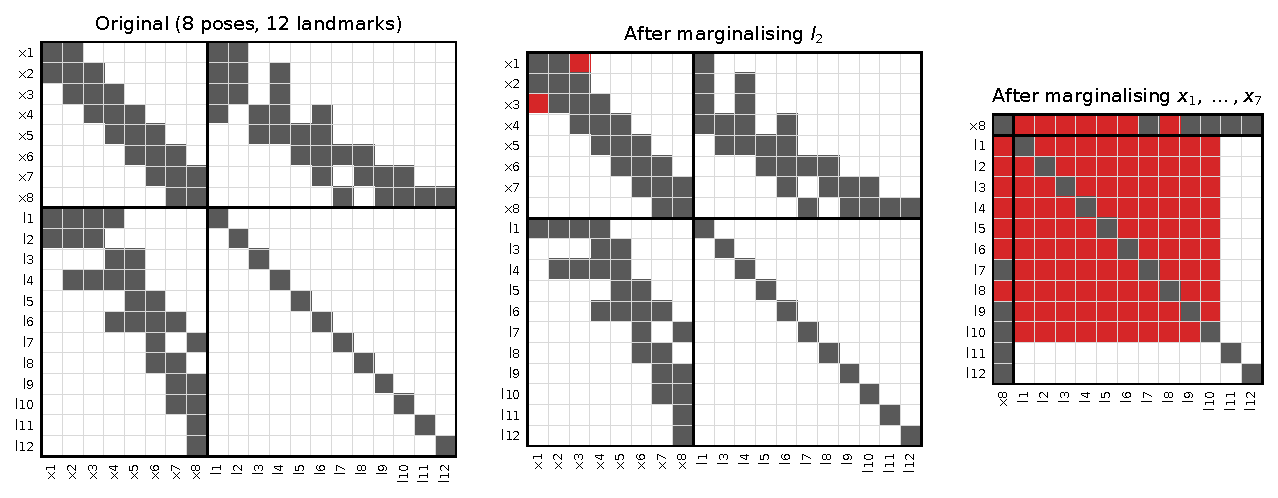
\includegraphics[width=\linewidth]{d1_spy_marginalization.pdf}
\caption{D1: block pattern of the handout matrix (left; poses $x$, landmarks $l$) and the
predicted pattern after marginalising $l_2$ (middle, question 6) and after marginalising
all past poses (right, question 7). Red blocks are fill-in created by the Schur complement.}
\label{fig:spy}
\end{figure}

\subsection{Deliverable 2: Well-begun is half done}\label{sec:d2}

\textbf{Proposal:} fix the root pose to the identity, compute a \emph{shortest-path
spanning tree} of the pose graph from the root (breadth-first search when all edges are
equally accurate; Dijkstra with edge weights equal to the measurement uncertainty, e.g.\
the trace of each edge's covariance, when they are not), and initialise every node by
composing the relative measurements along its tree path from the root.

\textbf{Rationale:} the initialisation error of a node grows with the number (and
uncertainty) of the measurements chained to reach it. Odometric chaining uses the path
$0\to1\to\dots\to i$, of length $i$. The shortest path also uses loop closures as
shortcuts, so on a graph with loops the hop count drops from $O(N)$ to the graph diameter,
and the accumulated noise drops with it. The method needs no special graph topology and
costs only $O(|\mathcal{E}|\log|\mathcal{V}|)$.

\subsection{Deliverable 3: Feature-based methods for SLAM (ORB-SLAM)}\label{sec:d3}

\paragraph{1. Modules (Fig.~1 of~\cite{murartal2015orb}).}
\begin{itemize}
\item \textbf{Map}: map points (3D position, viewing direction, representative ORB
  descriptor, scale-invariance range) and keyframes (pose, intrinsics, ORB features); the
  keyframes are connected by three graphs: the \emph{covisibility graph} (an edge when two
  keyframes share at least 15 map points), the \emph{spanning tree} and the sparse
  \emph{essential graph} (spanning tree, strong covisibility edges with at least 100
  shared points, and loop-closure edges).
\item \textbf{Place recognition}: a DBoW2 bag-of-words \emph{recognition database} of
  keyframes, built on an offline ORB \emph{visual vocabulary}; it is queried for
  relocalisation and for loop detection.
\item \textbf{Map initialisation}: computes a homography and a fundamental matrix in parallel
  from the first two frames, chooses one of them with a heuristic score, and builds the
  initial map by triangulation followed by full bundle adjustment.
\item \textbf{Tracking} (thread): extracts ORB features in every frame, estimates the
  camera pose from the previous frame with a constant-velocity model (or by global
  relocalisation when tracking is lost), refines it against the \emph{local map} (keyframes
  covisible with the current one) with motion-only BA, and decides whether to insert a new
  keyframe.
\item \textbf{Local mapping} (thread): processes new keyframes; it updates the covisibility
  graph, culls map points that are rarely found, triangulates new points from matches with
  covisible keyframes, runs \emph{local BA} on the current keyframe, its covisible keyframes
  and their points, and culls redundant keyframes (90\,\% of their points seen in at least
  three other keyframes).
\item \textbf{Loop closing} (thread): for each new keyframe, detects loop candidates with
  the bag-of-words database, computes the similarity transform $\mathrm{Sim}(3)$ to the loop
  keyframe (which also corrects scale drift), fuses the duplicated map points and
  corrects the poses on both sides of the loop, and finally optimises the \emph{essential
  graph} in $\mathrm{Sim}(3)$ to spread the loop correction over the whole map.
\end{itemize}

\paragraph{2. Wrong loop closures.}
ORB-SLAM accepts a loop only after several checks.
(i) \emph{Appearance}: a candidate keyframe must have a bag-of-words similarity higher than
the lowest similarity between the current keyframe and its covisible neighbours, and
keyframes already connected to the current one are excluded.
(ii) \emph{Temporal consistency}: a candidate is accepted only if three consecutive
keyframes produce loop candidates that are consistent, i.e.\ connected in the covisibility
graph.
(iii) \emph{Geometric verification}: ORB correspondences with the candidate are fed to
RANSAC with a $\mathrm{Sim}(3)$ solver (Horn's method); the transform is then refined, more
correspondences are searched with guided matching and the transform is optimised again. The
loop is accepted only with enough inliers (at least 40).

If a wrong loop passes these checks anyway, the method has no back-end mechanism to reject
it. The loop fusion merges map points that are actually different, and essential-graph
optimisation (a plain least-squares problem without robust kernels on the loop edges) pulls
the two places together. This bends and distorts the trajectory and the map
\emph{globally}. Later tracking and local BA are then done against a corrupted map, which
leads to more bad data associations and often to tracking failure. The error is not
undone later. This is why the checks above are very strict: ORB-SLAM gives up recall to
get near-perfect precision. Later systems added robust back-ends against outlier loops,
e.g.\ switchable constraints or pairwise consistency maximisation in Kimera-RPGO.

\subsection{Deliverable 4 (optional): Direct methods for SLAM (LSD-SLAM)}\label{sec:d4}

\paragraph{1. Modules of LSD-SLAM~\cite{engel2014lsd}.}
\begin{itemize}
\item \textbf{Tracking}: estimates the $\mathrm{SE}(3)$ pose of each new frame with respect to
  the current keyframe by minimising the variance-normalised photometric error over the
  pixels with depth (direct image alignment, Gauss--Newton on a pyramid).
\item \textbf{Depth map estimation}: refines the semi-dense inverse-depth map of the current
  keyframe with small-baseline stereo comparisons and filtering of tracked frames; when
  the camera moves too far, it creates a new keyframe by propagating the depth map to it.
\item \textbf{Map optimisation}: keyframes are added to a pose graph of $\mathrm{Sim}(3)$
  constraints, which come from direct $\mathrm{Sim}(3)$ image alignment between keyframes
  (with a depth residual, so scale drift is observable); the graph is optimised
  continuously in the background (g2o), and loop closures are found with FAB-MAP plus
  nearby keyframes.
\end{itemize}
\textbf{Similarities with ORB-SLAM:} keyframe-based design, separate tracking and mapping
threads, monocular input, $\mathrm{Sim}(3)$ pose graph to handle scale drift, appearance-based
loop detection with geometric verification. \textbf{Differences:} LSD-SLAM uses raw intensities
(photometric error) instead of ORB keypoints and reprojection error; it builds a
\emph{semi-dense} depth map (all pixels with enough gradient) instead of a sparse point map;
its back-end is a keyframe pose graph without bundle adjustment over the structure; and it
uses no descriptors, so its relocalisation is weaker.

\paragraph{2. Robustness.}
Feature-based methods are more robust to illumination changes and occlusions. Direct methods
assume brightness constancy: a change in exposure, auto-gain or lighting changes $I(p)$ and
biases the photometric error directly, unless one models affine brightness and calibrates
the camera photometrically as DSO does. Descriptors such as ORB/BRIEF use intensity
comparisons, which are invariant to monotonic brightness changes. Occluded points also simply fail to
match and are rejected by RANSAC or by robust kernels. In a direct method they become large
photometric residuals that enter a dense, non-convex alignment with a small convergence
basin. Direct methods are better in low-texture scenes and with motion blur, where keypoints
are scarce.

\subsection{Deliverable 5 (optional): From landmark-based SLAM to rotation estimation}\label{sec:d5}

\paragraph{Elimination of translations and landmarks.}
Since the Euclidean norm is invariant to rotations, $\|R_i^\top v\|=\|v\|$, so the first two
terms of problem~(1) are equal to
\begin{equation}
\sum_{(i,k)\in\mathcal{E}_l}\|p_k-t_i-R_i\bar p_{ik}\|_2^2
+\sum_{(i,j)\in\mathcal{E}_o}\|t_j-t_i-R_i\bar t_{ij}\|_2^2 .
\end{equation}
Stack the positions $x=[t_1^\top\cdots t_N^\top\ p_1^\top\cdots p_M^\top]^\top\in\mathbb{R}^{3(N+M)}$
and consider the graph whose nodes are poses and landmarks and whose $E=|\mathcal{E}_l|+|\mathcal{E}_o|$
edges are the observation and odometry edges. Let $A\in\mathbb{R}^{E\times(N+M)}$ be its
incidence matrix (row $e=(a,b)$ has $-1$ in column $a$ and $+1$ in column $b$) and
$\bar A=A\otimes I_3$. Each measured vector enters as $R_i\bar m_e$ with $\bar m_e\in\{\bar p_{ik},\bar t_{ij}\}$,
and $R_i\bar m_e=(\bar m_e^\top\otimes I_3)\,\mathrm{vec}(R_i)$ is linear in the rotations.
With $r=[\mathrm{vec}(R_1)^\top\cdots\mathrm{vec}(R_N)^\top]^\top\in\mathbb{R}^{9N}$ there is a
constant sparse matrix $B\in\mathbb{R}^{3E\times 9N}$ (row block $e$ has
$\bar m_e^\top\otimes I_3$ in the column block of the observing pose $i$) such that the
stacked measurements are $Br$. Problem~(1) becomes
\begin{equation}
\min_{R_i\in\mathrm{SO}(3)}\ \min_{x}\ \|\bar A x - Br\|_2^2 + \sum_{(i,j)\in\mathcal{E}_o}\|R_j-R_i\bar R_{ij}\|_F^2 .
\end{equation}
For fixed rotations the inner problem is an unconstrained \emph{linear} least-squares
problem in $x$ (the rotation term does not depend on $x$). Fixing the gauge ($t_1=0$, i.e.\
removing the first column block of $\bar A$, which leaves $\bar A$ with full column rank if
the graph is connected), its minimiser is
$x^\star(r)=(\bar A^\top\bar A)^{-1}\bar A^\top B r$, and the minimum value is
$\|(I-\bar A(\bar A^\top\bar A)^{-1}\bar A^\top)Br\|^2=r^\top B^\top \Pi B r$, where
$\Pi=I-\bar A(\bar A^\top\bar A)^{-1}\bar A^\top$ is the orthogonal projector onto the
complement of the range of $\bar A$ (the cycle space of the graph). Substituting back, we get
the rotation-only problem
\begin{equation}
\boxed{\ \min_{R_i\in\mathrm{SO}(3),\,i=1..N}\ r^\top Q\, r+\sum_{(i,j)\in\mathcal{E}_o}\|R_j-R_i\bar R_{ij}\|_F^2,\qquad Q=B^\top\Pi B\ }
\end{equation}
which depends on the rotations only. The original optimal translations and landmarks are
recovered in closed form as $x^\star(r^\star)$. The rotation term can also be written as a
quadratic form $r^\top (L_R\otimes I_3)\,r$ with a ``connection Laplacian'' of the odometry
graph, so the whole problem is $\min_{R\in\mathrm{SO}(3)^N} r^\top \tilde Q r$, a quadratic
problem over rotations.

\paragraph{Why the smaller problem is not necessarily faster.}
Optimisation-based SLAM is fast because its Hessian/information matrix is \emph{sparse}
(each measurement only involves two variables), so sparse Cholesky with a good ordering
solves each Gauss--Newton step in about linear time. Eliminating $x$ is a Schur complement
on all positions at once. As in D1.7, it connects every pair of poses joined by a path in
the graph: $\Pi$ (and hence $Q$) is in general \emph{dense}, and $(\bar A^\top\bar A)^{-1}$ is the
inverse of a graph Laplacian, which is dense for a connected graph. The rotation problem has
$9N$ instead of $3(N+M)+9N$ unknowns, but each iteration needs a dense $O(N^2)$ matrix and
$O(N^3)$ factorisation, while the original sparse problem costs about
$O(N+M)$--$O(N^{1.5})$. Forming $Q$ itself requires factorising $\bar A^\top\bar A$. Long
trajectories have thousands of poses, so the dense rotation-only problem is slower to solve
than the larger but sparse original.


\section{Team work}\label{sec:team}

\subsection{Setup}\label{sec:setup}

We used the provided Docker images \code{orbslam:latest} (ORB-SLAM3~\cite{campos2021orbslam3},
\code{Stereo-Inertial/\allowbreak stereo\_inertial\_euroc} with the stock \code{EuRoC.yaml}, Pangolin viewer
enabled by the lab patch) and \code{kimera:latest} (Kimera-VIO~\cite{rosinol2020kimera} pinned at
commit \code{980ff72d}, since the \code{feature/prerelease} branch no longer exists; lab
\code{params/} unchanged, loop closure detection off, \code{--initial\_k=50 --final\_k=10000}).
The dataset is EuRoC~\cite{burri2016euroc} \code{MH\_01\_easy} (3682 stereo pairs at 20\,Hz, IMU at
200\,Hz). The containers are started with \code{run\_docker\_vnav.sh}, which maps our container
paths to the docker host and forwards the X display. Both GUIs (Pangolin and Kimera's OpenCV
display) ran without errors. The two systems were run one after the other.

\textbf{One fix was needed for Kimera.} Kimera-VIO reads
\code{state\_groundtruth\_estimate0/\allowbreak sensor.yaml} with OpenCV's \code{FileStorage}, which only
accepts YAML files that start with \code{\%YAML:1.0}. The original EuRoC files do not have this
line, and the first run aborted with \emph{Cannot open file \dots/sensor.yaml}. We did not change
the SLAM code or the dataset. \code{scripts/run\_slam.sh} instead builds a hard-linked copy
\code{MH\_01\_easy\_kimera} (no extra disk space) in which only the \code{*.yaml} files get the
header, and runs Kimera on it with \code{run\_kimera.sh -p}.

Both runs covered the full sequence: ORB-SLAM3 output 3678 poses (one per frame, from $t_0$ to
the last image, 126 keyframes, a single map) and Kimera-VIO 818 keyframe poses (about 4.5\,Hz)
from frame 50 to the end. Then \code{fix\_timestamps.py} converted the ORB-SLAM3 stamps from
ns to s and Kimera's \code{traj\_vio.csv} to TUM format, and the ground truth was converted with
\code{evo\_traj euroc \dots --save\_as\_tum}. Plots come from \code{evo\_traj}~\cite{grupp2017evo}
with \code{--save\_plot} (no interactive window in our container), and the error statistics
come from \code{evo\_ape --align}. Timestamps are associated within 10\,ms; 3638 ORB-SLAM3 poses
and 813 Kimera poses fall inside the ground-truth interval. All commands are in
\code{scripts/evaluate.sh}, all numbers are in \code{results/d6/metrics.json}.

\subsection{Deliverable 6: trajectories without alignment}\label{sec:d6a}

\begin{figure}[tbp]
\centering
\begin{subfigure}[b]{0.48\linewidth}
  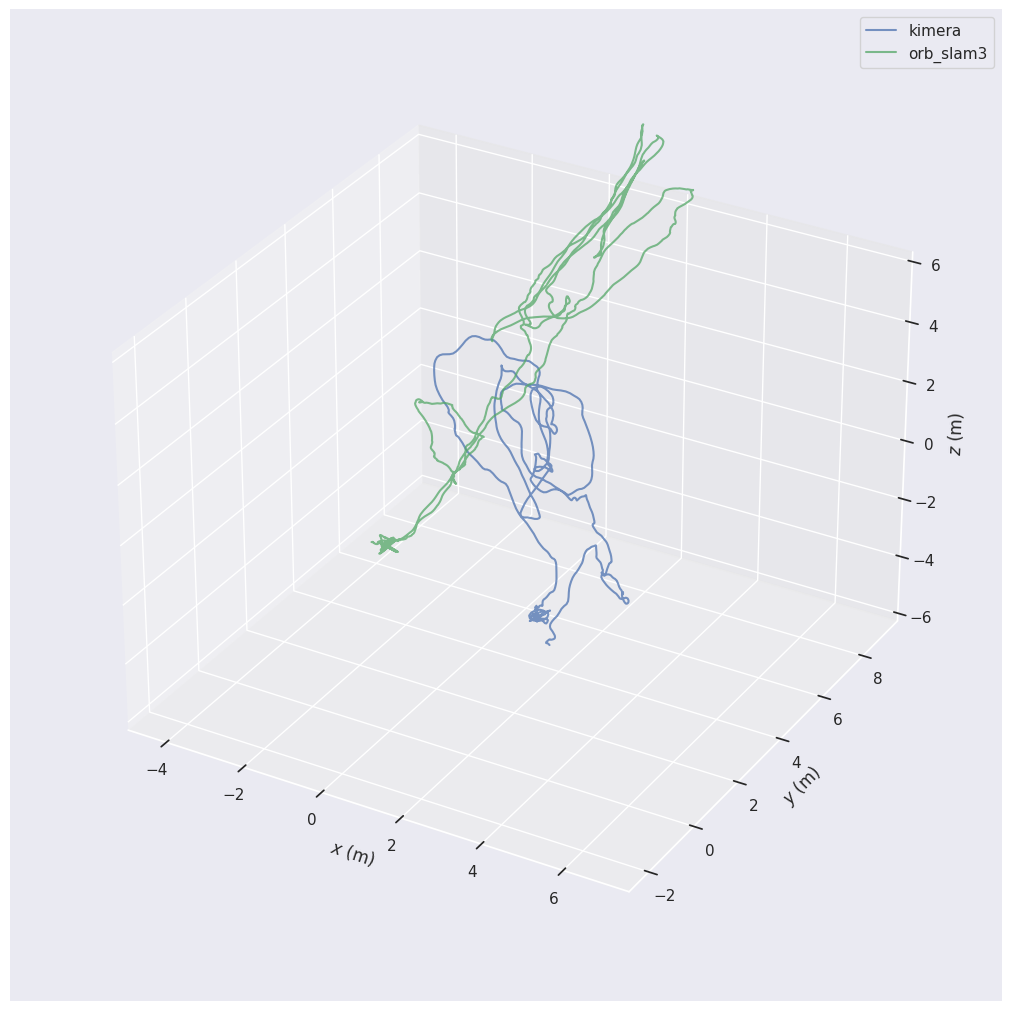
\includegraphics[width=\linewidth,trim=60 90 0 80,clip]{d6_evo_traj_unaligned.png}
  \caption{\code{evo\_traj tum kimera.txt orb\_slam3.txt --plot}}
\end{subfigure}

\vspace{0.4em}
\begin{subfigure}[b]{\linewidth}
  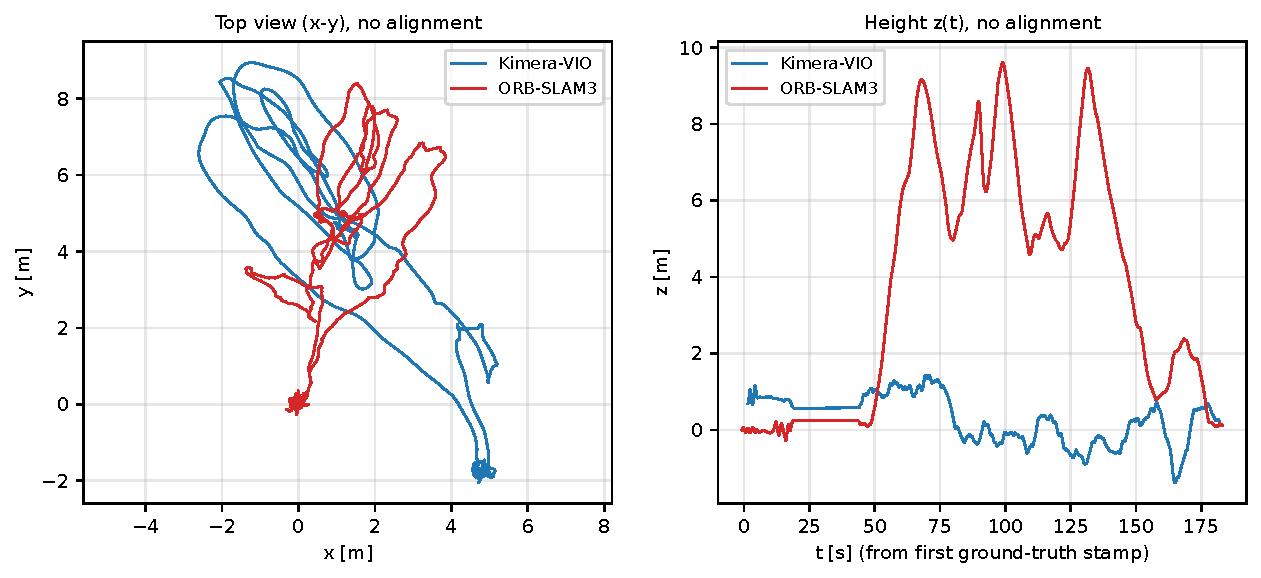
\includegraphics[width=\linewidth]{d6_unaligned.pdf}
  \caption{Same data: top view (dots mark the first pose) and height over time.}
\end{subfigure}
\caption{D6, no alignment: each trajectory is plotted in the world frame chosen by its own system.}
\label{fig:unaligned}
\end{figure}

\paragraph{What we see.} The two trajectories in Fig.~\ref{fig:unaligned} have the same length
(Kimera 79.1\,m, ORB-SLAM3 81.6\,m) and, after rotating one of them, the same shape, but they are
rotated, translated and tilted with respect to each other. Kimera starts at $(4.71,-1.79,0.69)$\,m
and moves in a nearly horizontal plane, with $z$ between $-1.3$ and $1.3$\,m. ORB-SLAM3 starts
exactly at the origin with identity orientation, and its ``height'' $z$ rises to 9.5\,m, which
the MAV did not fly: the motion that is horizontal in the real world appears along $z$ in the
ORB-SLAM3 frame. The two estimates are not wrong; they use \textbf{different world-frame
conventions}:
\begin{itemize}
\item \textbf{Kimera-VIO} initialises its state from the ground truth (\code{autoInitialize: 0}
  in \code{BackendParams.yaml}, which is why the run script passes \code{--log\_euroc\_gt\_data}):
  its first pose is the ground-truth pose of frame 50. Its world frame therefore \emph{is} the
  EuRoC (Vicon/Leica) world frame, with $z$ against gravity. After that point it is pure
  odometry.
\item \textbf{ORB-SLAM3} (stereo-inertial) estimates gravity during IMU initialisation, but
  its \code{SaveTrajectory\allowbreak EuRoC} function writes every pose relative to the IMU pose of the \emph{first
  keyframe} ($T_{w b_0}^{-1} T_{w b_k}$). Its world frame is thus the body frame of the
  vehicle at start-up. In EuRoC the IMU $x$ axis points roughly up, so gravity is along
  $(-0.94,\,0.05,\,0.34)$ in this frame; the frame is tilted by $110^\circ$ with respect to
  the ground truth and its origin is the starting position.
\end{itemize}
Because the frames differ by a rigid transformation that is not observable from the data
(a VIO system can observe roll and pitch from gravity, but the global yaw and position are
unobservable and fixed by convention), a meaningful comparison needs an alignment step.

\subsection{Deliverable 6: trajectories aligned with ground truth}\label{sec:d6b}

\begin{figure}[tbp]
\centering
\begin{subfigure}[b]{0.48\linewidth}
  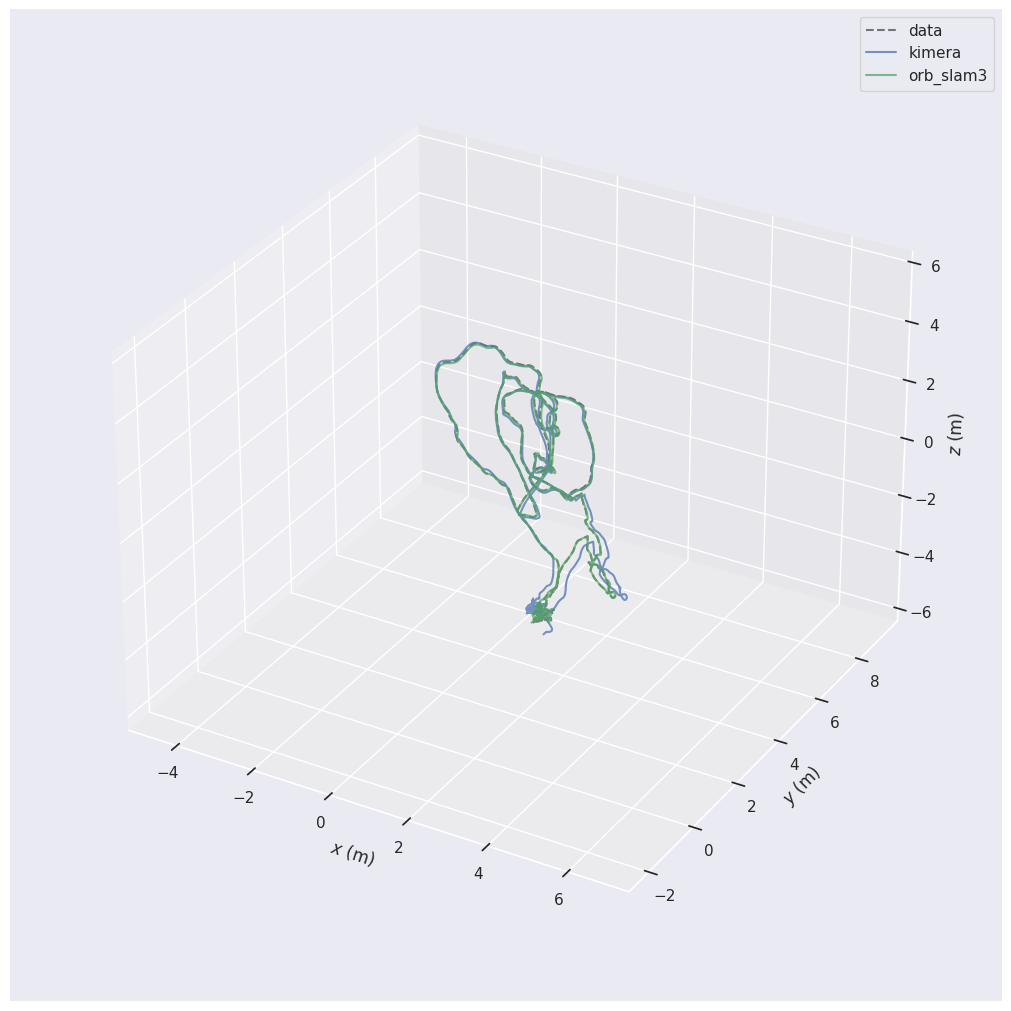
\includegraphics[width=\linewidth,trim=60 90 0 80,clip]{d6_evo_traj_aligned.png}
  \caption{\code{evo\_traj \dots --ref data.tum --plot --align}}
\end{subfigure}

\vspace{0.4em}
\begin{subfigure}[b]{\linewidth}
  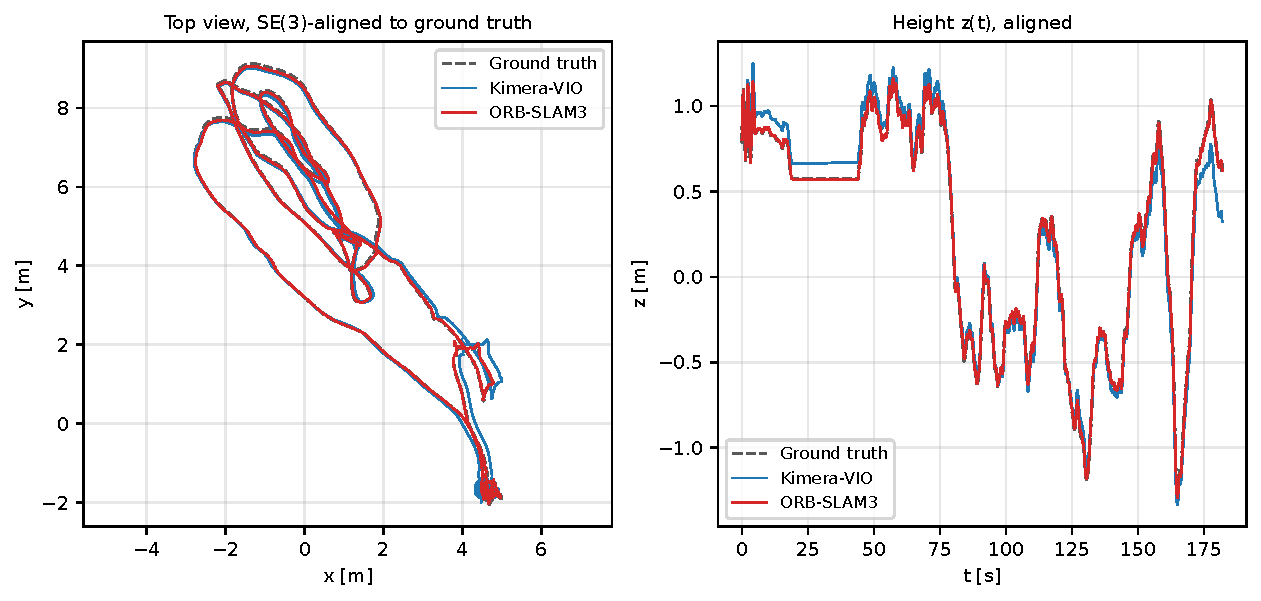
\includegraphics[width=\linewidth]{d6_aligned.pdf}
  \caption{Same data: top view and height, ground truth dashed.}
\end{subfigure}

\vspace{0.4em}
\begin{subfigure}[b]{\linewidth}
  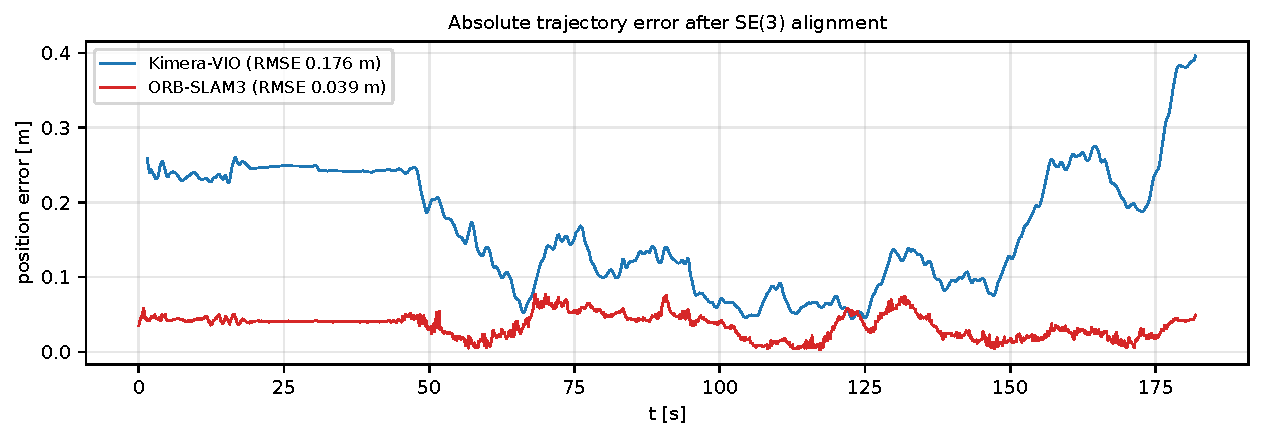
\includegraphics[width=\linewidth]{d6_ate_time.pdf}
  \caption{Position error over time after the $\mathrm{SE}(3)$ alignment (\code{evo\_ape --align}).}
\end{subfigure}
\caption{D6, after $\mathrm{SE}(3)$ alignment (Umeyama~\cite{umeyama1991}, no scale) of each estimate to the
EuRoC ground truth.}
\label{fig:aligned}
\end{figure}

\code{--align} solves for the rigid transformation $T\in\mathrm{SE}(3)$ that minimises
$\sum_k\|T p^{\text{est}}_k - p^{\text{gt}}_k\|^2$ over all associated positions. For Kimera this transformation is
almost the identity ($1.8^\circ$ of tilt, $0.3^\circ$ of yaw, 0.23\,m of translation), as expected
from its ground-truth initialisation. For ORB-SLAM3 it is the $110^\circ$ rotation plus the
$(4.67,-1.74,0.87)$\,m offset to the starting point. After alignment both trajectories lie on
top of the ground truth (Fig.~\ref{fig:aligned}), including the height profile, and the
differences are now visible only in the error plot and in Table~\ref{tab:ate}.

\begin{table}[H]
\centering\small
\begin{tabular}{lcc}
\toprule
 & Kimera-VIO & ORB-SLAM3 \\
\midrule
poses evaluated (rate) & 813 (keyframes, $\approx$4.5\,Hz) & 3638 (every frame, 20\,Hz)\\
ATE RMSE, $\mathrm{SE}(3)$ align [m] & 0.176 & \textbf{0.039} \\
ATE mean / median / max [m] & 0.157 / 0.136 / 0.396 & \textbf{0.035 / 0.040 / 0.077} \\
rotation error RMSE [deg] & 2.54 & \textbf{1.25} \\
ATE RMSE, $\mathrm{Sim}(3)$ align [m] & 0.170 & \textbf{0.021} \\
estimated scale factor $s$ & 1.011 & 1.008 \\
end-point error, first pose aligned [m] & 0.62 (0.78\,\% of path) & \textbf{0.018} \\
max.\ error, first pose aligned [m] & 0.62 (at the end) & 0.16 \\
\bottomrule
\end{tabular}
\caption{Accuracy on the full \code{MH\_01\_easy} sequence (\code{evo\_ape}, translation part unless
stated; \code{results/d6/evo/ape\_*.txt}, \code{results/d6/metrics.json}).}
\label{tab:ate}
\end{table}

\paragraph{Drift.} Kimera-VIO is visual-inertial \emph{odometry}: a fixed-lag smoother
(iSAM2 over the last 25 keyframes, i.e.\ about 5\,s) with structureless stereo smart factors and
IMU preintegration~\cite{forster2017preintegration}. Information older than the horizon is
marginalised, and features are never matched against the old part of the map. Yaw and
position errors therefore accumulate. With only the first pose aligned, its error grows
monotonically and reaches its maximum, 0.62\,m, at the very end. The global $\mathrm{SE}(3)$
alignment hides part of this by distributing the drift over the trajectory. This is why the
aligned error in Fig.~\ref{fig:aligned}c is about 0.25\,m in the first 50\,s, while the MAV is
still near the start, drops in the middle of the run and rises again to 0.40\,m at the end.
ORB-SLAM3 has a constant error of about 4\,cm with no growth over time: its first-pose-aligned
error stays below 0.16\,m everywhere and returns to 1.8\,cm at the end, when the MAV is back near
its take-off point.

\paragraph{Loop closure vs.\ map re-use.} Kimera-VIO was run as pure VIO (\code{USE\_LCD=0},
i.e.\ without Kimera-RPGO), so it has no mechanism to correct past drift. ORB-SLAM3 is a full
SLAM system with place recognition, loop closing and map merging. In this run, however, its
log shows no loop or merge event: a single map with 126 keyframes was kept for the whole
sequence. Its drift-free result comes from \emph{mid-term data association}. When the MAV
returns to an area it already mapped (\code{MH\_01} flies over the same parts of the machine
hall several times and ends near the start), tracking matches the current frame against the
existing map points of covisible keyframes, and local visual-inertial BA ties the new keyframes
to the old ones. The drift is corrected before it can grow, so the loop never needs to be
``closed'' explicitly. On a longer sequence with a real loop the loop-closing thread and the
global BA would also be used.

\paragraph{Scale.} Both systems observe metric scale from the stereo baseline (11\,cm) and the
accelerometer, so neither should have scale drift. A $\mathrm{Sim}(3)$ alignment confirms this:
the estimated scale factors are 1.008 (ORB-SLAM3) and 1.011 (Kimera), and correcting scale
reduces the ATE by only 0.6\,cm for Kimera. The 1.8\,cm reduction for ORB-SLAM3 is a
noticeable fraction of its very small error, but it is still under 1\,\% of scale. This is
different from monocular systems such as LDSO (Section~\ref{sec:d7}), whose trajectories have
an arbitrary scale and need \code{--correct\_scale}.

\paragraph{Other differences.} (i) Kimera publishes only keyframe poses, so its curve is
sparser; ORB-SLAM3 writes a pose for every frame. (ii) ORB-SLAM3's trajectory starts
0.9\,s before the ground truth and Kimera's 1.5\,s after it (Kimera skips the first 50
frames), so evo evaluates slightly different time intervals; this has no effect on the
comparison above. (iii) Kimera's rotation error is twice that of ORB-SLAM3 (2.5$^\circ$ vs
1.3$^\circ$). Its yaw drift is the main source of its position error, because a yaw error
$\delta\psi$ moves a point at distance $d$ by about $d\,\delta\psi$, and the hall is about
10\,m across. (iv) The two systems also do different amounts of work: Kimera processed the
sequence in 46\,s ($\approx 4\times$ faster than real time) while drawing its 3D mesh, and
ORB-SLAM3 ran at about real time.

\subsection{Deliverable 7 (optional): LDSO}\label{sec:d7}

\paragraph{Setup.} LDSO~\cite{gao2018ldso} is DSO~\cite{engel2018dso} (direct, sparse,
monocular) with ORB-feature place recognition (DBoW3) and a $\mathrm{Sim}(3)$ pose graph for
loop closure. We built the upstream master (\code{9b0c48c}) unmodified, together with its
bundled DBoW3 and g2o. Pangolin v0.6 is the only extra dependency and was installed in a
local prefix (\code{scripts/build\_ldso.sh}). We ran it as in the handout,
\code{run\_dso\_euroc preset=0 files=\dots/mav0/cam0}, i.e.\ on the left camera only, with
the radial-tangential calibration shipped in \code{examples/EUROC/EUROC.txt} and without
photometric calibration, which EuRoC does not provide (\code{scripts/run\_ldso.sh}). The Pangolin
viewer worked. All 3682 frames were processed, without tracking loss, and LDSO kept 711
keyframes. It ran single-threaded and slower than real time (about 16 min with the GUI). The
place-recognition module accepted \textbf{16 loop closures}, for example keyframe 134$\to$97,
571$\to$427 and 684$\to$216, and at the end of the sequence 687--697$\to$5--10, when the MAV
returns to its take-off area. LDSO writes two trajectories, with and without the loop-closure
pose graph (\code{results.txt} and \code{results.txt.noloop}). Both are clean TUM files with
timestamps in seconds; our \code{fix\_ldso.py} found no malformed lines to drop. Because
LDSO is monocular, all trajectories are aligned with $\mathrm{Sim}(3)$
(\code{evo\_traj \dots --align --correct\_scale --plot\_mode xy}).

\begin{figure}[tbp]
\centering
\begin{subfigure}[b]{0.36\linewidth}
  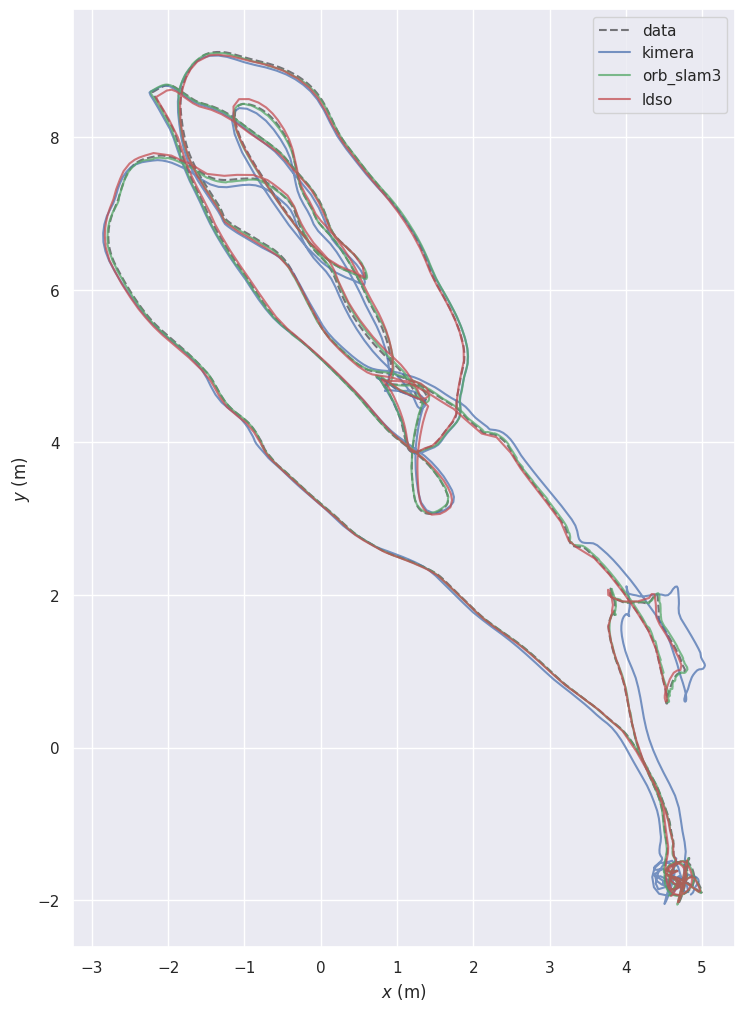
\includegraphics[width=\linewidth]{d7_evo_traj_sim3_xy.png}
  \caption{\code{evo\_traj} (\code{--align --correct\_scale --plot\_mode xy}).}
\end{subfigure}\hfill
\begin{subfigure}[b]{0.62\linewidth}
  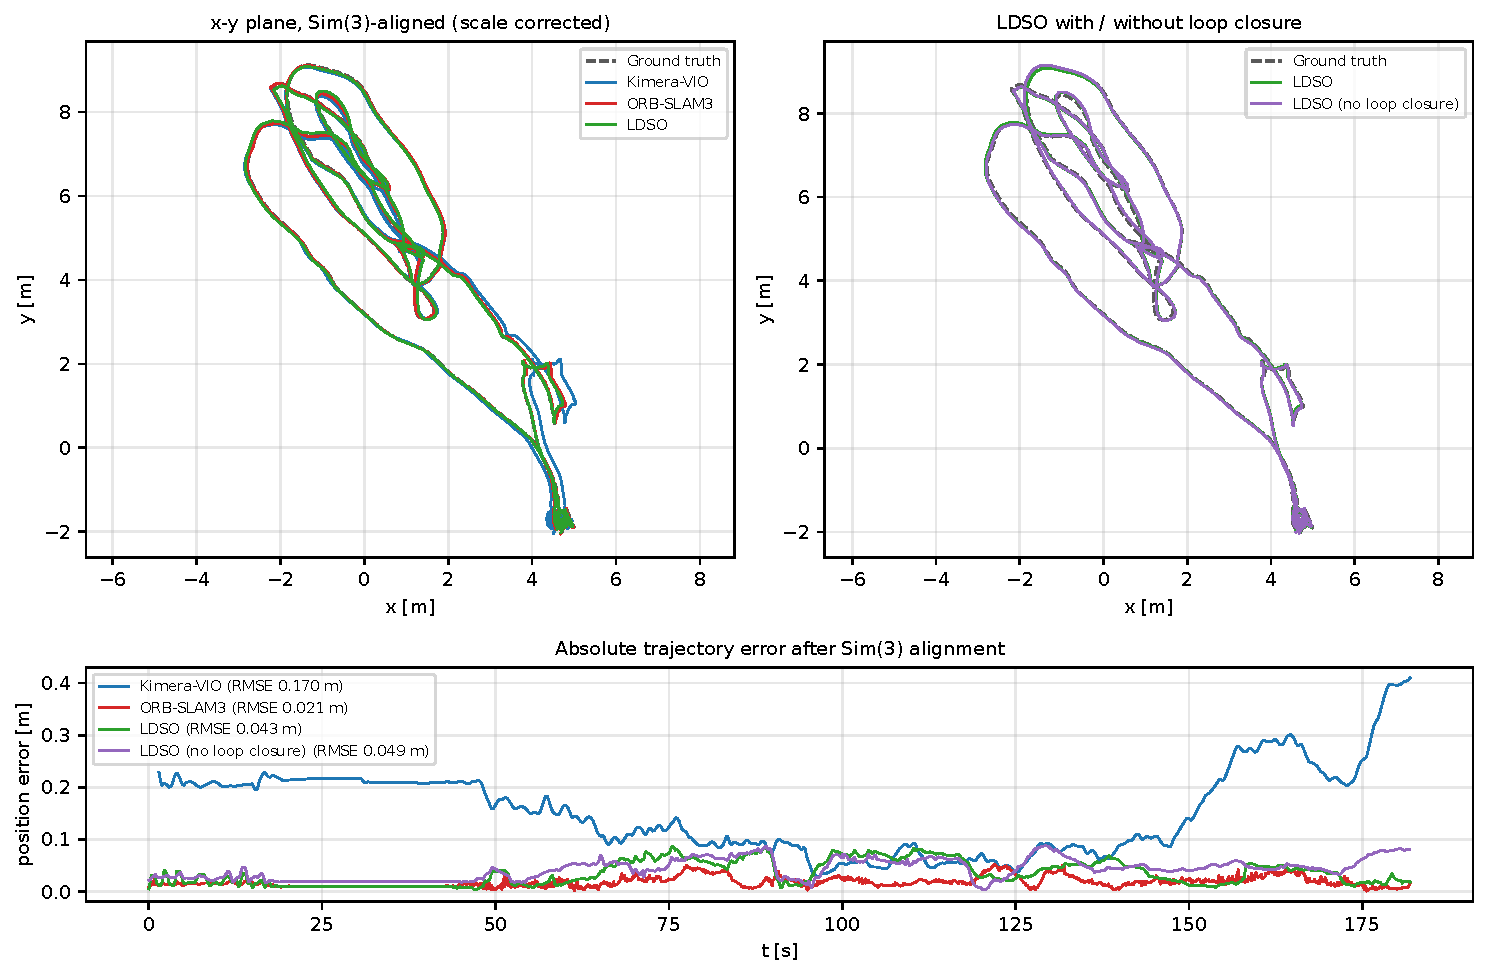
\includegraphics[width=\linewidth]{d7_sim3_aligned.pdf}
  \caption{Same alignment: x-y plane, LDSO with/without loop closure, and error over time.}
\end{subfigure}
\caption{D7: Kimera-VIO, ORB-SLAM3 and LDSO on \code{MH\_01\_easy}, each $\mathrm{Sim}(3)$-aligned
to the ground truth.}
\label{fig:d7}
\end{figure}

\begin{table}[tbp]
\centering\small
\begin{tabular}{lcccc}
\toprule
 & Kimera-VIO & ORB-SLAM3 & LDSO & LDSO, no loop \\
\midrule
sensors & stereo + IMU & stereo + IMU & mono & mono \\
poses evaluated & 813 & 3638 & 696 & 696 \\
raw path length [m] (GT 80.6) & 79.1 & 81.6 & 52.2 & 52.3 \\
$\mathrm{Sim}(3)$ scale factor $s$ & 1.011 & 1.008 & 1.524 & 1.534 \\
ATE RMSE, $\mathrm{Sim}(3)$ [m] & 0.170 & \textbf{0.021} & 0.043 & 0.049 \\
ATE max, $\mathrm{Sim}(3)$ [m] & 0.410 & \textbf{0.052} & 0.086 & 0.088 \\
ATE RMSE, $\mathrm{SE}(3)$ only [m] & 0.176 & 0.039 & 1.570 & 1.590 \\
\bottomrule
\end{tabular}
\caption{D7 accuracy on the full sequence (\code{results/d7/metrics.json},
\code{results/d7/evo/ape\_*\_sim3.txt}).}
\label{tab:d7}
\end{table}

\paragraph{Differences between the trajectories.}
\begin{itemize}
\item \textbf{Scale.} The raw LDSO trajectory is 52\,m long instead of 80.6\,m: a monocular
  system can only recover the trajectory up to an unknown global scale, which DSO fixes
  arbitrarily during initialisation. Evo has to stretch it by $s=1.52$. Without scale
  correction ($\mathrm{SE}(3)$ only) the LDSO error is 1.57\,m, which only reflects the wrong
  scale and says nothing about the shape. The two stereo-inertial systems need $s\approx1.01$.
\item \textbf{Shape after $\mathrm{Sim}(3)$ alignment.} LDSO follows the ground truth closely
  (4.3\,cm RMSE). It is about $4\times$ better than Kimera-VIO (17.0\,cm) and about half as
  accurate as ORB-SLAM3 (2.1\,cm). In Fig.~\ref{fig:d7}a it is hard to tell LDSO and ORB-SLAM3
  apart, while Kimera's yaw drift is visible on the right-hand part of the hall (around
  $x\approx4$--5\,m), where Kimera is offset from the other two. The comparison favours LDSO
  somewhat: $\mathrm{Sim}(3)$ alignment gives it a free scale parameter, and its error is
  evaluated only at its 696 keyframes. Even so, on this well-textured, well-lit sequence the
  direct photometric front-end is very accurate.
\item \textbf{Effect of loop closure.} The trajectories with and without loop closure almost
  overlap (Fig.~\ref{fig:d7}b). Loop closure reduces the RMSE from 4.9 to 4.3\,cm, and mostly
  helps at the end of the sequence: without loops the error grows to 8\,cm in the last
  20\,s, while the loops to keyframes 5--10 bring the end of the trajectory back onto the
  start. The scale also changes slightly (1.534$\to$1.524), because the $\mathrm{Sim}(3)$ pose
  graph corrects scale drift as well. The improvement is small because DSO's odometry drifts
  little on \code{MH\_01}: the sequence is short, slow and well textured. Loop closure matters
  much more on longer trajectories.
\item \textbf{Frames and timing.} Like ORB-SLAM3, LDSO starts at the identity in its own
  frame (here the first camera frame, $z$ along the optical axis), so without alignment it
  would be rotated and scaled with respect to both other trajectories. It outputs only
  keyframes (711, about 3.9\,Hz).
\end{itemize}

\section{Conclusions}
The information-matrix exercises show that marginalisation always fills in the matrix
among the neighbours of the eliminated variable, which is why fixed-lag smoothers and filters
become dense while full smoothing stays sparse. On EuRoC \code{MH\_01\_easy}, the raw
trajectories of ORB-SLAM3 and Kimera-VIO cannot be compared directly, because each system
picks its own world frame. After an $\mathrm{SE}(3)$ alignment, ORB-SLAM3 is about $4.5\times$ more
accurate (3.9\,cm vs 17.6\,cm ATE RMSE). The difference comes from map re-use rather than from
the front-end: Kimera-VIO is odometry and drifts by 0.8\,\% of the travelled distance, while
ORB-SLAM3 keeps re-observing its old map and has no measurable drift. Both recover the true
metric scale. The monocular direct method LDSO cannot recover scale (factor 1.52). Once scale is
corrected, its shape is accurate to 4.3\,cm, and loop closure only helps it slightly on this short,
well-textured sequence.

\section*{Individual responsibility}
Team: Team Fullcans. The individual deliverables D1--D5 are answered in
Section~1, and the team deliverables D6 and D7 (optional, LDSO) in Section~2.

\bibliographystyle{unsrtnat}
\bibliography{references}

\end{document}
